\section{Harun Ar - Rasyid(1174027)}
\subsection{Pengertian}
Geografi adalah ilmu pengetahuan yang mengambarkan segala sesuatu yang ada di permukaan bumi. \hfill\break
Geografi juga selain mempelajari bagian permukaan bumi, tapi juga mempelajari seluruh bagian bumi mulai darti struktur bumi,jenis batuan yang menyusun bumi serta atmosfer yang melindungi bumi. \hfill\break
Segala aktifitas yang terjadi di bumi merupakan bagian dari ilmu Geografi.\hfill\break
\subsection{Sejarah}
Sejarah geografi dimulai sejak manusia mulai berinteraksi dengan lingkunganya, hal ini juga merupakan awal mula dari berkembangnya ilmu pengetahuan tentang geografi.\hfill\break
Pada awalnya geografi hanya membahas atau mendekripsikan gambaran umum tentang fakta-fakta yang menjelaskan keadaan di muka bumi. Pada abad ke-18 yaitu masa geografi klasik, ilmu geografi hanya sebatas menjelaskan dan mengumpulkan informasi tentang lingkungan geografi saja, misalnya: keadaan politik, industri, iklim terutama di kota-kota besar.\hfill\break
Sejarah geografi terus berjalan dan berkembang. Tepatnya, diabad ke-19 geografi mengalami perkembangan dari segi keilmuannya. Dari yang semula hanya mendeskripsikan saja kemudian berkembang menjadi lebih spesifik yaitu dengan menjelaskan lingkungan geografi secara sistematis.\hfill\break
Pada pertengahan abad ke-19, keilmuan dalam geografi sudah membahas sampai ketingkat membandingkan keadaan, data geografis dan karakteristik antara wilayah yang satu dengan wilayah yang lain di muka bumi. Hal ini kita kenal sebagai “Comparative Geography”.\hfill\break
Perkembangan keilmuwan geografi semakin pesat pasca terjadinya perang dunia ke-II. Yang semula dikembangkan oleh imuwan Amerika dan Inggris yang dikenal sebagai “Comparative Geography” kemudian berkembang menjadi “Global Geography” dimana objek kajiannya semakin luas yaitu meliputi seluruh dunia. Era inilah yang dinamakan sebagai “era geografi modern”.\hfill\break
Dari pembahasan di atas, kita sudah mengetahui kapan sejarah geografi itu dimulai yaitu sejak adanya interaksi antara manusia dengan lingkungannya. Bila seperti itu, maka hakekatnya sejak Nabi Adam as turun ke bumi sebetulnya geografi sudah ada.\hfill\break
Akan tetapi penggalian geografi secara keilmuan sendiri baru dilakukan pertama kali oleh orang-orang Yunani. Dimana pada perkembangan awalnya dilatarbelakangi oleh suatu upaya masyarakat Yunani untuk melepaskan diri dari alam pikiran dan kepercayaan. Dimana kepercayaan tersebut meyakini bahwa dewa-dewa ikut turut campur dalam segala bentuk kejadian di bumi.\hfill\break
Istilah geografi sebenarnya baru digunakan pada tahun 1972 sedangkan sebelumnya lebih menggunakan istilah “ilmu bumi”. Istilah ini pertama kali diperkenalkan oleh seorang ahli filsafat dan astronomi yang bernama Eratosthenes pada 276 194 sebelum masehi.Kemudian, Claudius Ptoleumaeus melakukan peletakan dasar-dasar keilmuan geografi.\hfill\break
Sejarah perkembangan geografi terus berlanjut. Immanuel Kant mengembangkan geografi modern kemudian Karl Ritter juga mengembangkan geografi sosial.\hfill\break
Selain itu ada tokoh-tokoh lain yang ikut andil dalam mengembangkan geografi yaitu Alexander von Humbolt sebagai peletak dasar geografi fisika modern dan sebagainya.\hfill\break
\subsection{Koordinat}
Koordinat didapatkan dari hasil perpotongan antara garis latitude (Y) / lintang dan garis longitude(X) / garis bujur sehingga bisa menunjukan suatu lokasi pada suatu daerah. \hfill\break 
Umumnya koordinat dibedakan menajadi koordinat Geografi dan Universal Transver Mercator(UTM). Pada koordinat geografi dibedakan menajadi 3 yaitu : \hfill\break
\begin{itemize}
	\item Degree, Decimal(DD, DDDD) contoh S 4.56734 E 102.67235
	\item Degree,Minute(DD MM,MMMM) contoh S 4 42,5423’ E 105 34,6445’
	\item Degree, Minute, Second(DD MM SS,SS) contoh : S 4 43’ 45,22 E 103 33’ 33,25
\end{itemize}
\hfill\break
\begin{figure}[H]
	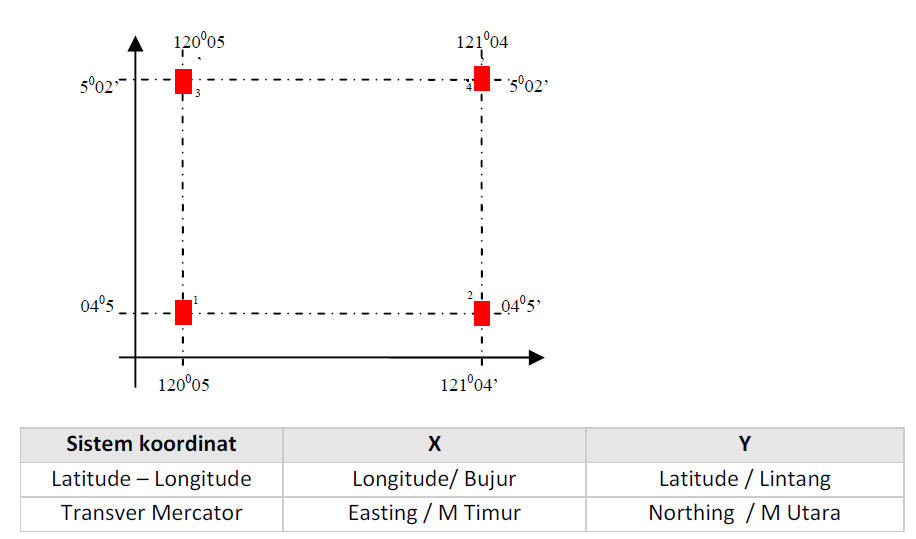
\includegraphics[width=4cm]{figures/1174027/1_1174027_koordinat.jpg}
	\centering
	\caption{Contoh Koordinat}
\end{figure}
Pada system koordinat UTM biasanya terdapat pembagian waktu berdasarkan zonasinya. \hfill\break
\begin{figure}[H]
	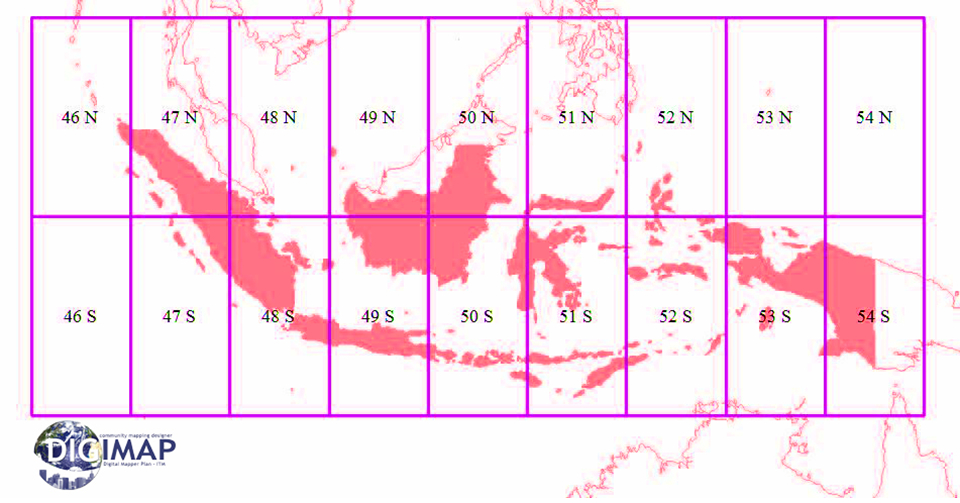
\includegraphics[width=4cm]{figures/1174027/1_1174027_UTM.jpg}
	\centering
	\caption{Contoh Koordinat UTM}
\end{figure}

\subsection{Data Geospasial}
Data geospasial merupakan pengambaran lokasi geografis,dimensi atau ukuran / karakteristik objek alam atau buatan manusia yang berada di bawah atau di atas permukaan bumi, data geospasial biasanya di singkat menjadi DG.
\hfill\break
Data Geospasial dibagi menjadi 2 yaitu :
\begin{itemize}
	\item Vektor
	Vektor merupakan salah jenis gambar yang dapat dibuat menggunakan aplikasi corel / adobe illustrator / aplikasi vektor lainnya. \hfill\break 
	Vektor itu sering digunakan untuk membuat gambar animasi dan vektor juga digunakan oleh goole maps.
	\item Roshen
	Roshen merupakan gambar yang di ambil dari satelit di luar angkasa, gambar ini biasanya bertipe jpg, dan pembaharuan data gambar ini berlangsung lama karena proses nya yang memakan waktu cukup banyak, jenis data ini digunakan oleh google earth.
\end{itemize}
\subsection{Link}
\begin{itemize}
	\item \href{https://youtu.be/mhk9PhmNLvk}{Pengertian GIS}
	\item \href{https://youtu.be/7K0x-oQncy4}{Sejarah GIS}
	\item \href{https://youtu.be/QE8uvqNqbo4}{Koordinat}
	\item \href{https://youtu.be/CXYenLiAS8U}{Data Geospasial}
\end{itemize}
\subsection{Plagiarism}
\begin{figure}[H]
	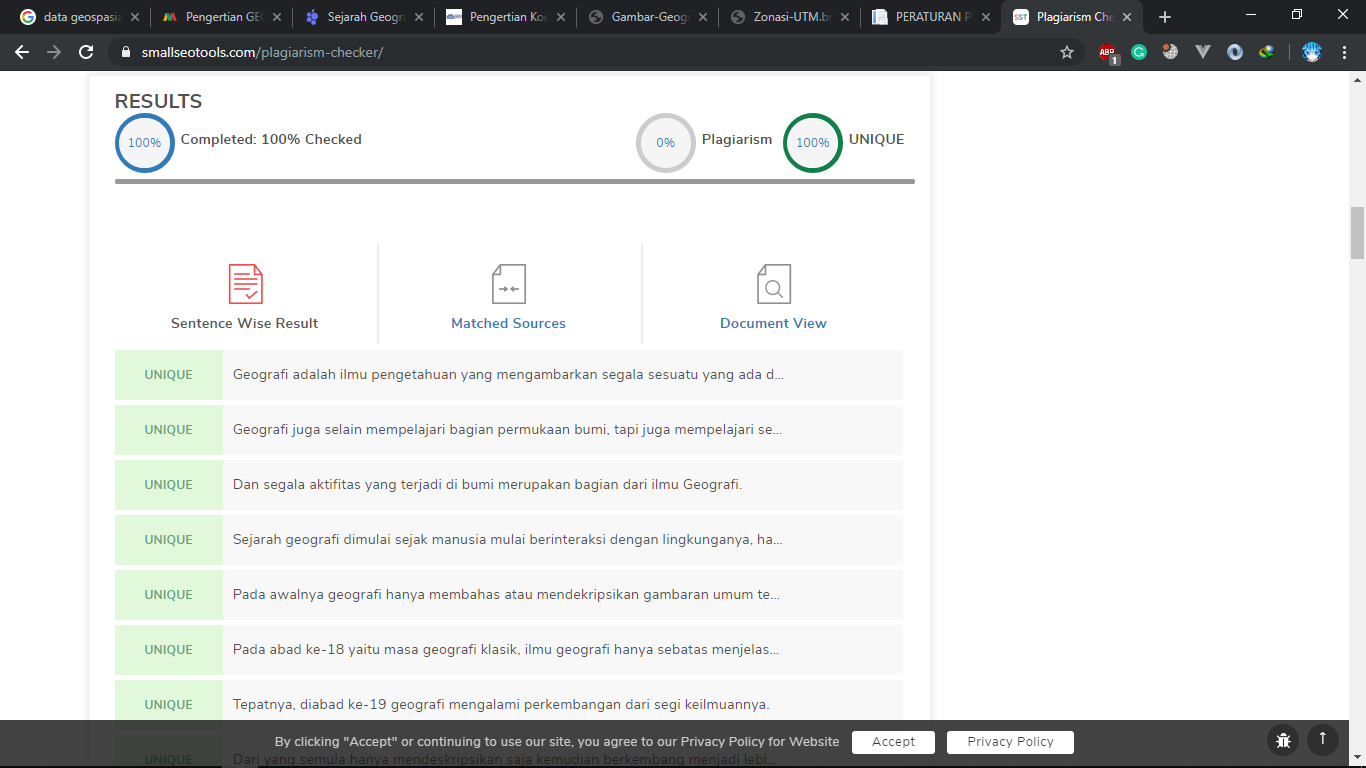
\includegraphics[width=4cm]{figures/1174027/1_1174027_placek.png}
	\centering
	\caption{Bukti Tidak Melakukan Plagiat}
\end{figure}